\documentclass[pdflatex,compress,mathserif]{beamer}

%\usetheme[dark,framenumber,totalframenumber]{ElektroITK}
\usetheme[darktitle,framenumber,totalframenumber]{ElektroITK}

\usepackage[utf8]{inputenc}
\usepackage[T1]{fontenc}
\usepackage{lmodern}
\usepackage[bahasai]{babel}
\usepackage{amsmath}
\usepackage{amsfonts}
\usepackage{amssymb}
\usepackage{graphicx}
\usepackage{multicol}

\newcommand*{\Scale}[2][4]{\scalebox{#1}{$#2$}}%

\setbeamertemplate{caption}[numbered]
\setbeamertemplate{section in toc}[sections numbered]

\title{Sinyal dan Sistem}
\subtitle{Sinyal dan Sistem}

\author{Mifta Nur Farid, S.T., M.T.}

\begin{document}

\maketitle

\section{Sinyal sinusoidal waktu kontinu}
\begin{frame}{Sinyal sinusoidal waktu kontinu}
	\begin{figure}
		\centering
		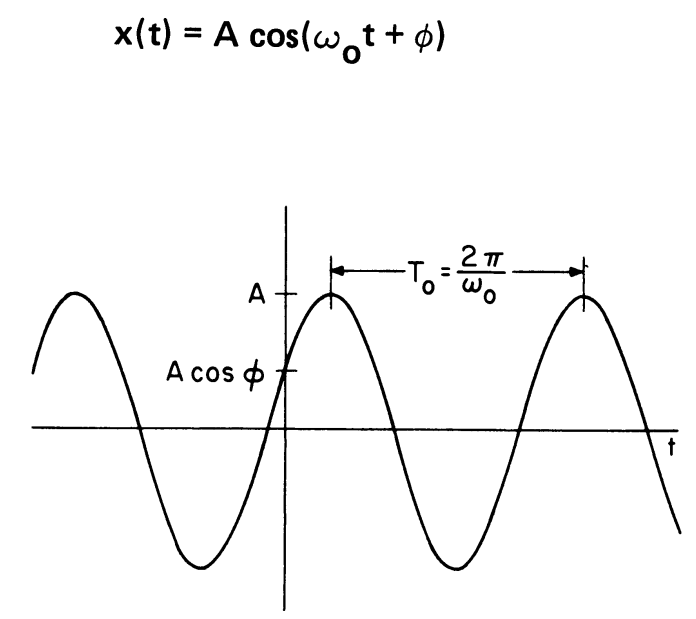
\includegraphics[height=0.8\textheight]{img/01.slide_01}
	\end{figure}
\end{frame}

\begin{frame}{Sinyal sinusoidal waktu kontinu}
	\begin{figure}
		\centering
		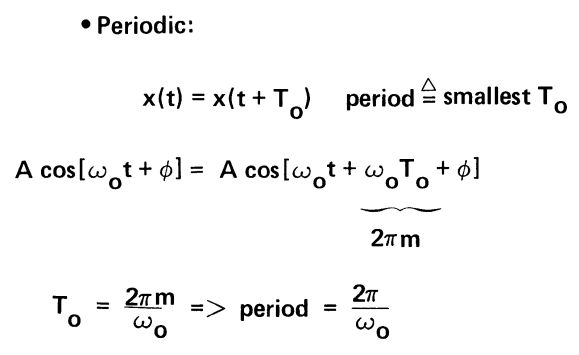
\includegraphics[height=0.7\textheight]{img/01.slide_02_01}
	\end{figure}
\end{frame}

\begin{frame}{Sinyal sinusoidal waktu kontinu}
	\begin{figure}
		\centering
		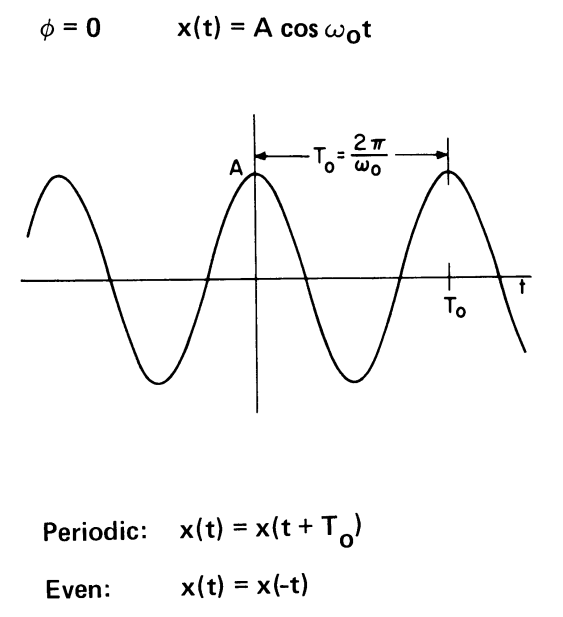
\includegraphics[height=0.8\textheight]{img/01.slide_03}
	\end{figure}
\end{frame}

\begin{frame}{Sinyal sinusoidal waktu kontinu}
	\begin{figure}
		\centering
		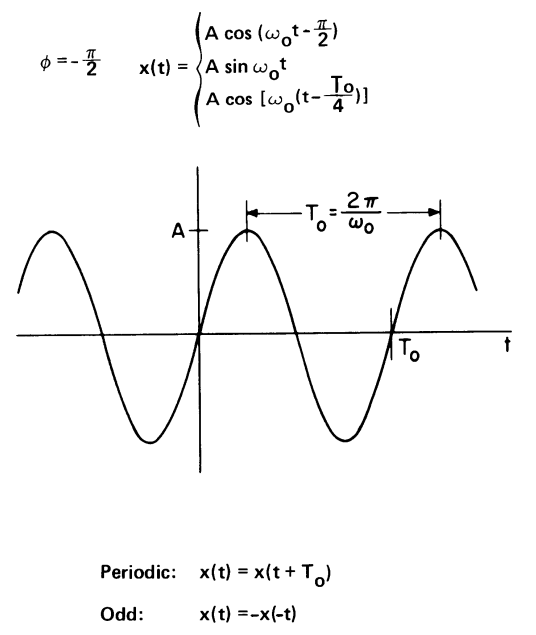
\includegraphics[height=0.8\textheight]{img/01.slide_04}
	\end{figure}
\end{frame}

\section{Sinyal sinusoidal waktu diskret}
\begin{frame}{Sinyal sinusoidal waktu diskret}
	\begin{figure}
		\centering
		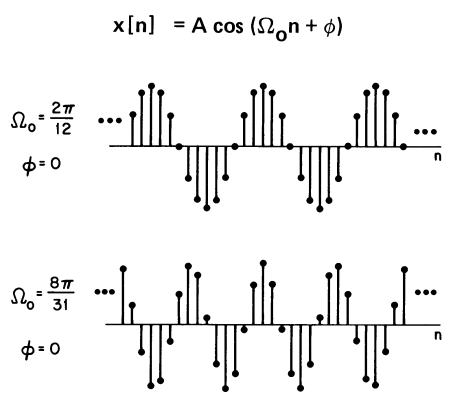
\includegraphics[height=0.8\textheight]{img/01.slide_05}
	\end{figure}
\end{frame}

\begin{frame}{Sinyal sinusoidal waktu diskret}
	\begin{figure}
		\centering
		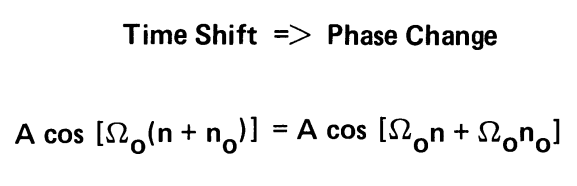
\includegraphics[height=0.3\textheight]{img/01.slide_06}
	\end{figure}
\end{frame}

\begin{frame}{Sinyal sinusoidal waktu diskret}
	\begin{figure}
		\centering
		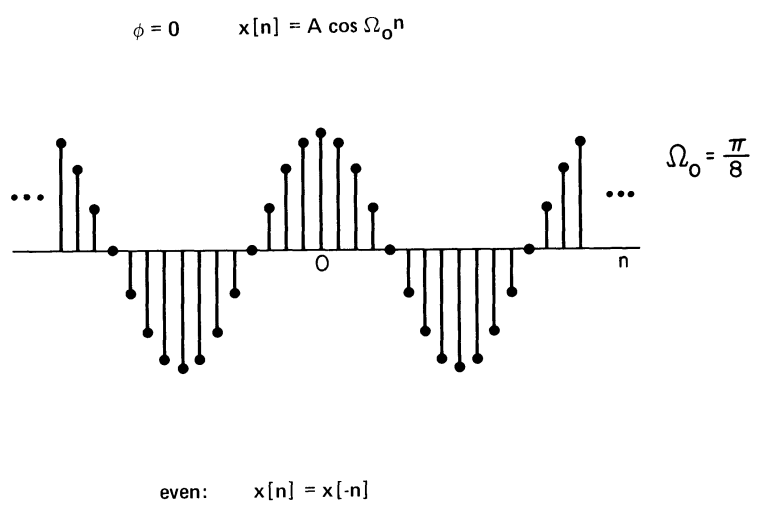
\includegraphics[height=0.8\textheight]{img/01.slide_07}
	\end{figure}
\end{frame}

\begin{frame}{Sinyal sinusoidal waktu diskret}
	\begin{figure}
		\centering
		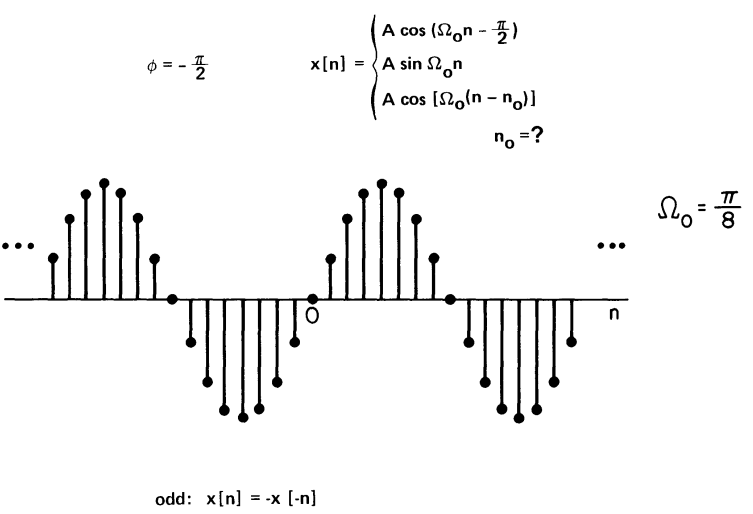
\includegraphics[height=0.8\textheight]{img/01.slide_08}
	\end{figure}
\end{frame}

\begin{frame}{Sinyal sinusoidal waktu diskret}
	\begin{figure}
		\centering
		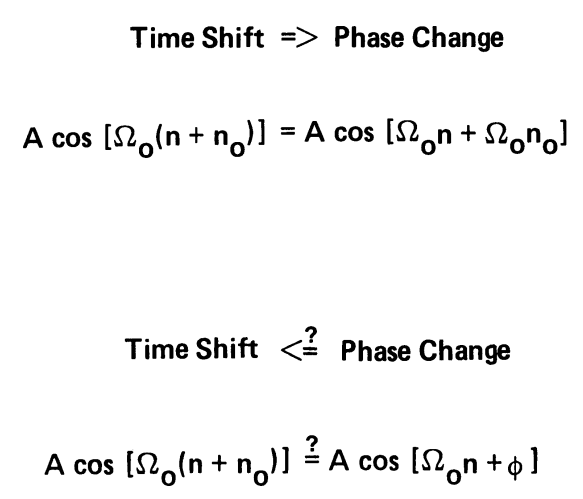
\includegraphics[height=0.8\textheight]{img/01.slide_09}
	\end{figure}
\end{frame}

\begin{frame}{Sinyal sinusoidal waktu diskret}
	\begin{figure}
		\centering
		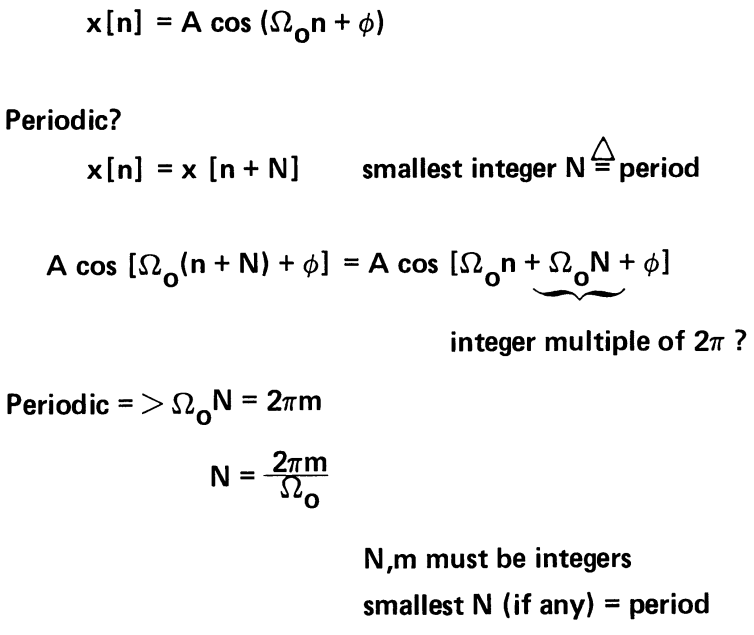
\includegraphics[height=0.8\textheight]{img/01.slide_10}
	\end{figure}
\end{frame}

\begin{frame}{Sinyal sinusoidal waktu diskret}
	\begin{figure}
		\centering
		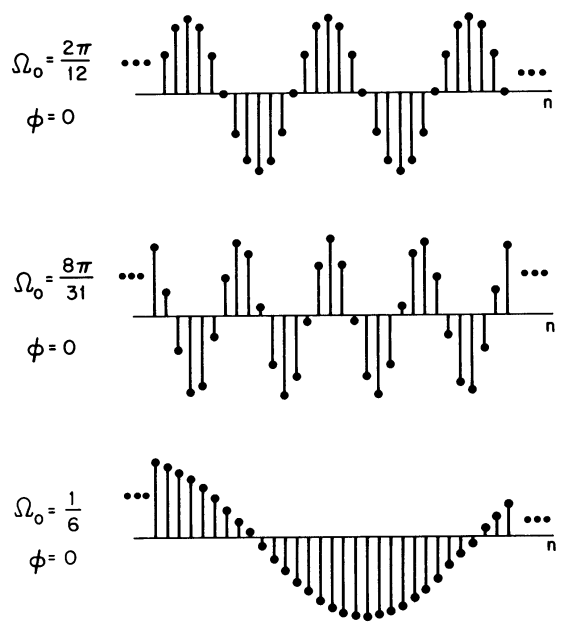
\includegraphics[height=0.8\textheight]{img/01.slide_11}
	\end{figure}
\end{frame}

\begin{frame}{Sinyal sinusoidal waktu diskret}
	\begin{figure}
		\centering
		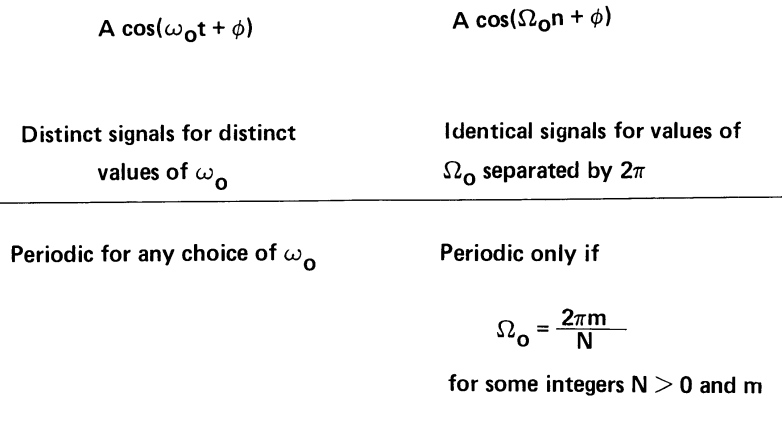
\includegraphics[height=0.8\textheight]{img/01.slide_12}
	\end{figure}
\end{frame}

\section{Sinyal sinusoidal saat frekuensinya berbeda}
\begin{frame}{Sinyal sinusoidal saat frekuensinya berbeda}
	\begin{figure}
		\centering
		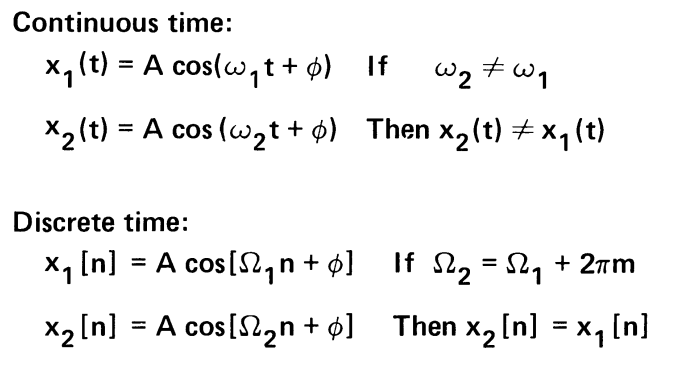
\includegraphics[height=0.8\textheight]{img/01.slide_13}
	\end{figure}
\end{frame}

\section{Sinyal eksponensial riil waktu kontinu}
\begin{frame}{Sinyal eksponensial riil waktu kontinu}
	\begin{figure}
		\centering
		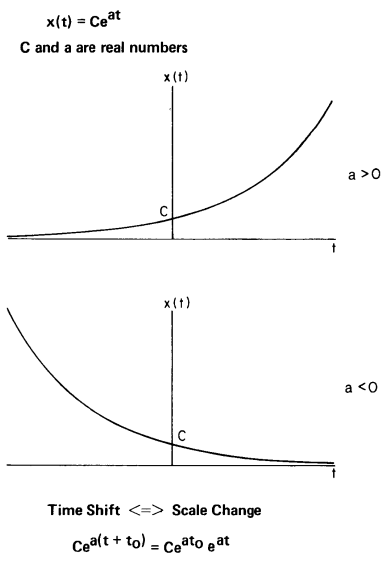
\includegraphics[height=0.8\textheight]{img/01.slide_14}
	\end{figure}
\end{frame}

\section{Sinyal eksponensial riil waktu diskret}
\begin{frame}{Sinyal eksponensial riil waktu diskret}
	\begin{figure}
		\centering
		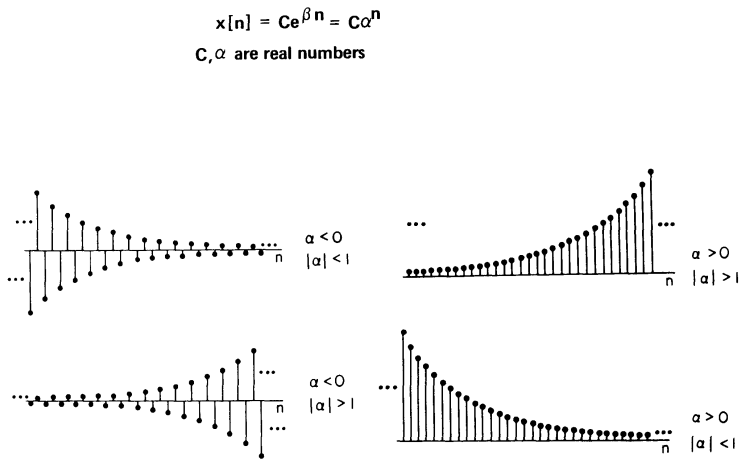
\includegraphics[height=0.8\textheight]{img/01.slide_15}
	\end{figure}
\end{frame}

\section{Sinyal eksponensial kompleks waktu kontinu}
\begin{frame}{Sinyal eksponensial kompleks waktu kontinu}
	\begin{figure}
		\centering
		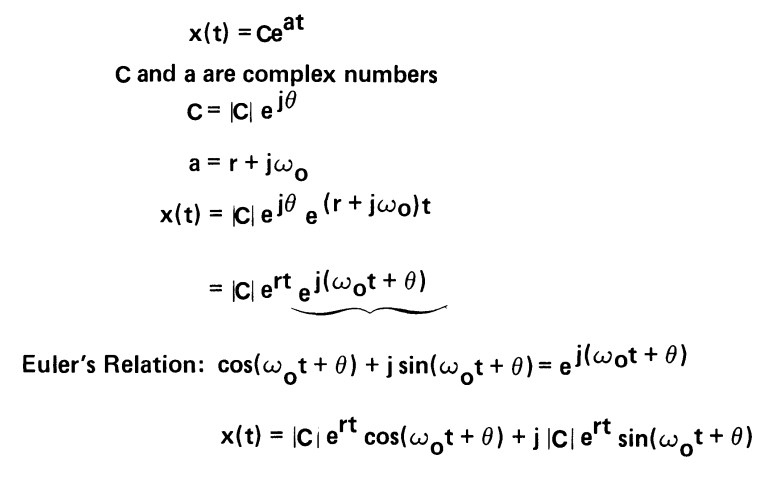
\includegraphics[height=0.8\textheight]{img/01.slide_16}
	\end{figure}
\end{frame}

\begin{frame}{Sinyal eksponensial kompleks waktu kontinu}
	\begin{figure}
		\centering
		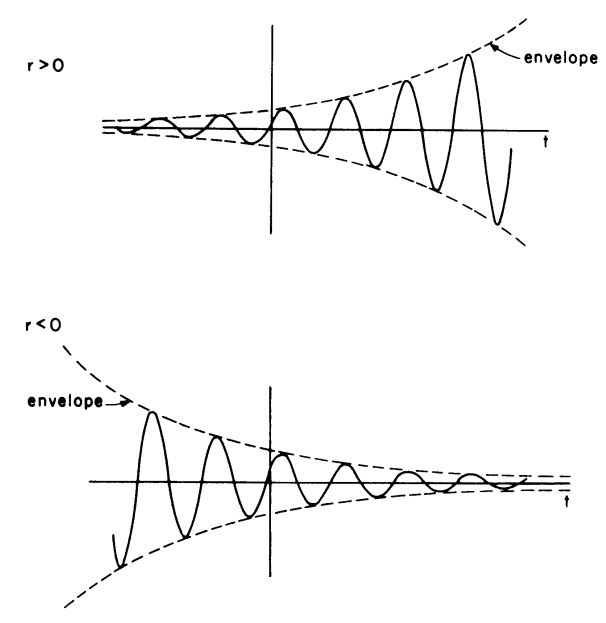
\includegraphics[height=0.8\textheight]{img/01.slide_17}
	\end{figure}
\end{frame}

\section{Sinyal eksponensial kompleks waktu diskret}
\begin{frame}{Sinyal eksponensial kompleks waktu diskret}
	\begin{figure}
		\centering
		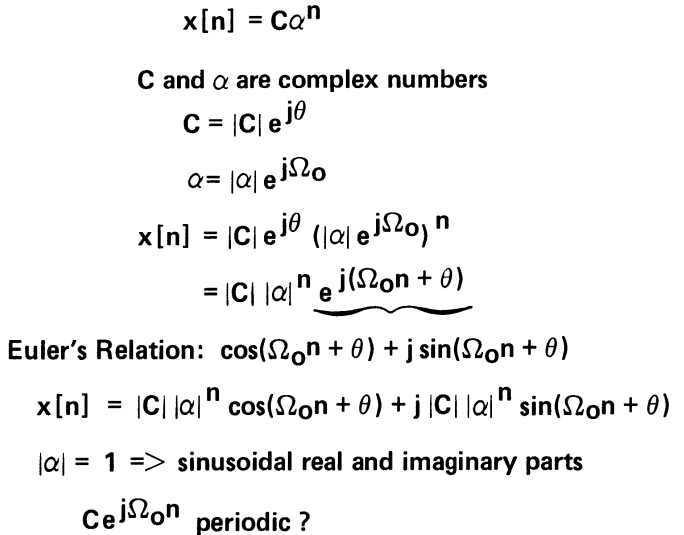
\includegraphics[height=0.8\textheight]{img/01.slide_18}
	\end{figure}
\end{frame}

\begin{frame}{Sinyal eksponensial kompleks waktu diskret}
	\begin{figure}
		\centering
		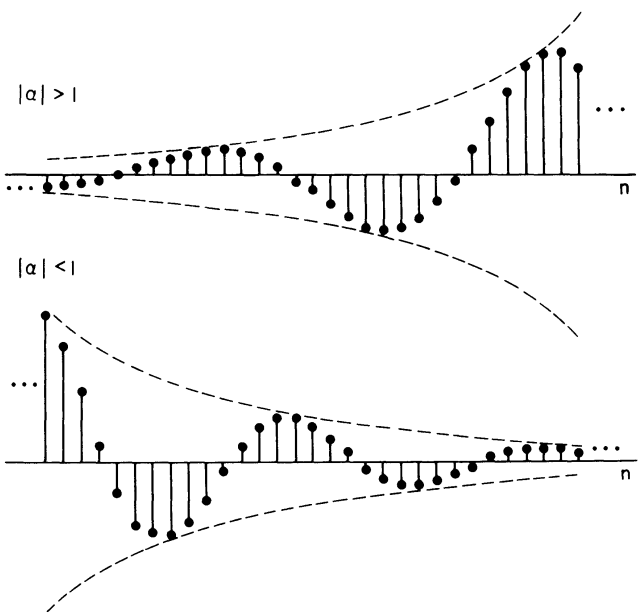
\includegraphics[height=0.8\textheight]{img/01.slide_19}
	\end{figure}
\end{frame}

\section{Unit Step \& Unit Impulse}
\begin{frame}{Unit Step \& Unit Impulse}
	\begin{figure}
		\centering
		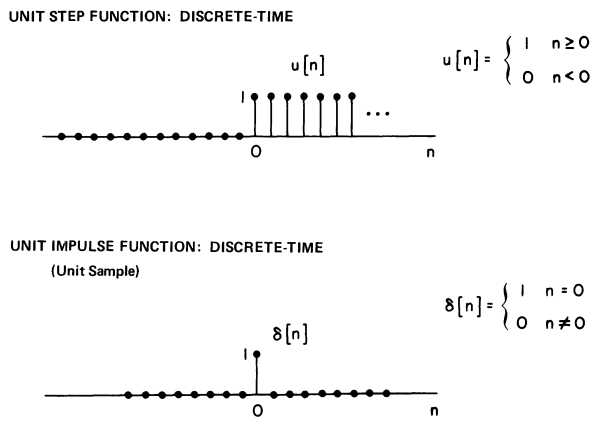
\includegraphics[height=0.8\textheight]{img/02.slide_01}
	\end{figure}
\end{frame}

\begin{frame}{Unit Impulse Sequence}
	\begin{figure}
		\centering
		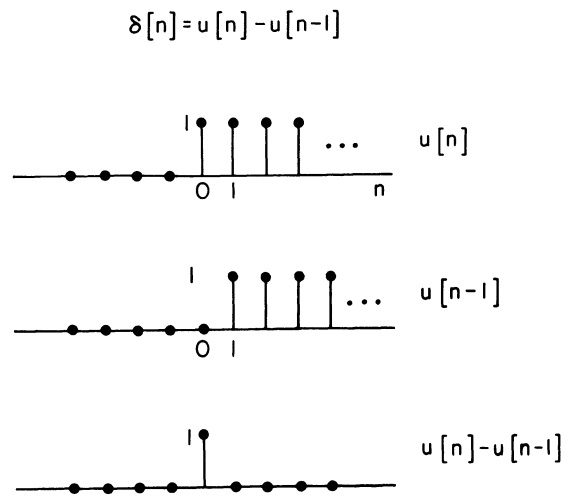
\includegraphics[height=0.8\textheight]{img/02.slide_02}
	\end{figure}
\end{frame}

\begin{frame}{Unit Step Sequence}
	\begin{figure}
		\centering
		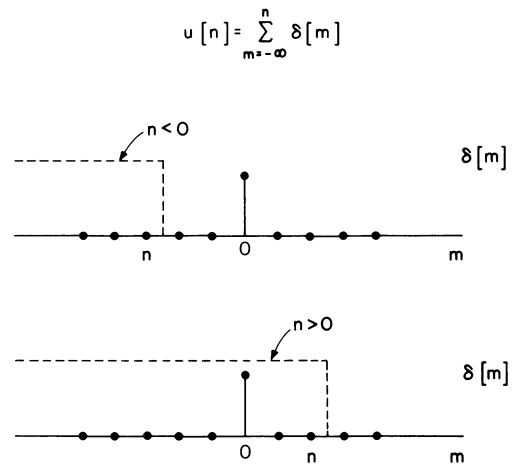
\includegraphics[height=0.8\textheight]{img/02.slide_03}
	\end{figure}
\end{frame}

\begin{frame}{Unit Step Sequence}
	\begin{figure}
		\centering
		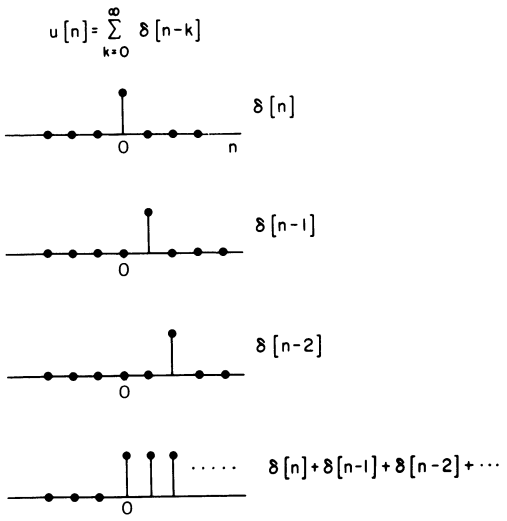
\includegraphics[height=0.8\textheight]{img/02.slide_04}
	\end{figure}
\end{frame}

\begin{frame}{Unit Step Function Waktu Kontinu}
	\begin{figure}
		\centering
		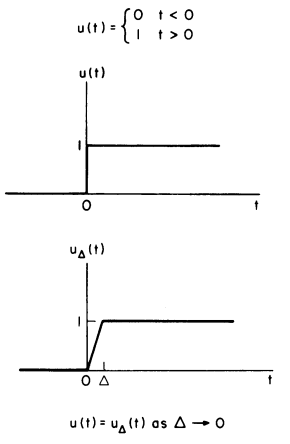
\includegraphics[height=0.8\textheight]{img/02.slide_05}
	\end{figure}
\end{frame}

\begin{frame}{Unit Impulse Function}
	\begin{figure}
		\centering
		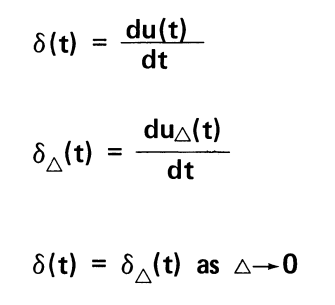
\includegraphics[height=0.4\textheight]{img/02.slide_06}
	\end{figure}
\end{frame}

\begin{frame}{Unit Impulse Waktu Kontinu}
	\begin{figure}
		\centering
		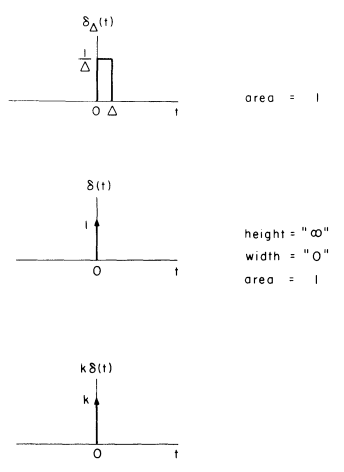
\includegraphics[height=0.8\textheight]{img/02.slide_07}
	\end{figure}
\end{frame}

\begin{frame}{Unit Step Waktu Kontinu}
	\begin{figure}
		\centering
		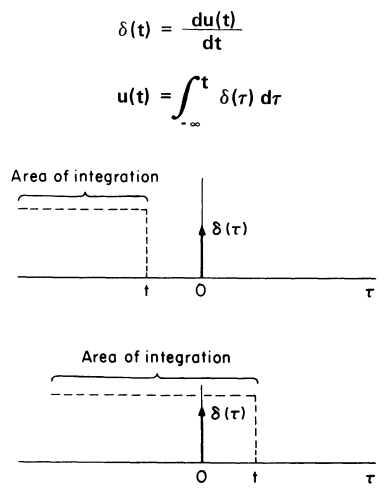
\includegraphics[height=0.8\textheight]{img/02.slide_08}
	\end{figure}
\end{frame}

\section{Bahan Bacaan Mandiri}

\begin{frame}
	\frametitle{Bahan Bacaan Mandiri}
	\begin{enumerate}
		\item Oppenheim, A. V., Willsky, A. S. \& Nawab, S. H., (1997). Signal and Systems, Second Edition. New Jersey: Prentice Hall of India.
		\begin{itemize}
			\item Section 1.1, Transformations of the independent variable, pp. 7-11
			\item Section 1.3.1, Continuous-time complex exponential and sinusoidal signals, pp. 15-21
			\item Section 1.3.2, Discrete-time complex exponential and sinusoidal signals, pp. 21-25
			\item Section 1.3.3, Periodicity properties of discrete-time complex exponentials, pp. 25-30
		\end{itemize}
	\end{enumerate}
\end{frame}
\end{document}
